This chapter presents a loopless Gray code for generating all ordered trees with $n$ nodes. 
Sections \ref{sec:otree-otherresults} and \ref{sec:termsandcons} give context on this Gray code's relationship to related results and discuss terminology for this chapter's results. Section \ref{sec:otree-successor} provides a 2-case successor rule for the algorithm; Section \ref{sec:otree-proof} gives a proof of our algorithm's correctness.

% Section \ref{sec:otree-otherresults} gives context on this Gray code's relationship to related results, section \ref{sec:termsandcons} discuss terminology for this chapter's results, section \ref{sec:otree-successor} provides a 2-case successor rule for the algorithm, and section \ref{sec:otree-proof} gives a proof of our algorithm's correctness.
% Cooldyck was first loopless for Dyck and Binary; we now show also ordered
% Give exampl  of bit change that messup tree (show for bin and o). 
% \chapter{Test}

\section{Relationship to Previous Results} \label{sec:otree-otherresults}
Ruskey and Williams previously gave a Gray code for generating all Dyck words of a given length in cool-lex order via prefix shifts \cite{ruskey2008generating}.  In the same paper, Ruskey and Williams also gave a Gray code for generating all binary trees with a fixed number in the same order, making the cool-lex order of Dyck words a simultaneous Gray code for Dyck words of order $n$ and binary trees with $n$ nodes.

% TODO: adaptation of order, new successor rule
This thesis provides a new Gray code that generates another Catalan object, ordered trees, with a fixed number of nodes in a cool-lex order using \emph{pops} and \emph{pushes}.  These pop and push operations remove a node's first child (pop) and push a node to be another node's new first child (push).  Our Gray code generates all ordered trees using at most 2 pushes and 2 pops per generated tree. This constitutes the first pop-push Gray code for ordered trees.  Additionally, the algorithm generates a minimal change ordering of ordered trees in the same order as their corresponding Dyck words in Ruskey and Williams's algorithm for Dyck words and binary trees. Therefore, in conjunction with the result from \cite{ruskey2008generating}, the cool-lex order for Dyck words now creates a simultaneous Gray code for Dyck words, binary trees, and ordered trees.  As we will see in chapter \ref{chap:otree-implementation}, this Gray code can be implemented via a looples algorithm like the the cool-lex algorithms for Dyck words and binary trees. 


\section{Terminology and Conventions} \label{sec:termsandcons}

Throughout this chapter, we typeset ordered trees as $\tree{T}$, and we use $n$ to denote the number of nodes in a tree.
We typeset nodes of a tree as $X$, and we frequently refer to a node and the subtree rooted at that node interchangeably.
Code is written with a \texttt{monospaced} font.

When discussing an ordered tree $\tree{T}$, we use the term \emph{first branching}, which could be misinterpreted. 
We use the term to mean the following: 
The first branching occurs when the preorder traversal goes up an edge, and then down an edge, for the first time.
The node that is incident to both of these edges is the parent of the first branching.
% For example, these first branches are highlighted in turquoise in Figure \ref{fig:trees6}.
In particular, note that the subtree to the left of the first branch must be a path (see Remark \ref{rem:left-is-path}). Moreover, note that the first branching is also the first time a second child is visited in a preorder traversal of $\tree{T}$.  All previously visited nodes in a preorder traversal are either the root or the first child of their parent.

% Another way of describing the first branching is as follows.  Let $\leftpath{T}$ be the unique path between 

Another way of describing the first branching is as follows.
Let $O$ be the first second-child node that is visited during a preorder traversal.
If $P$ is the parent of $O$, then $P$ is the parent of the first branching.
We frequently label the following nodes around the first branching: $O$ and $P$ are defined as above; $L$ is $P$'s first child, and $G$ is $P$'s parent. 
Fig. \ref{fig:exampleotree} gives an example illustrating an ordered tree's first branching and the nodes $O,P,G,$ and $L$. In the special case that $\tree{T}$ has no first branching, and therefore $\tree{T}$ is a path, we define $O$ to be $\tree{T}$'s unique leaf.

% The number of ordered trees with $n$ nodes is the $(n-1)$st Catalan number, $\C_{n-1}$.



% Let $F$ be the leftmost leaf of T, or equivalently the leftmost descendant of the root. Consider the unique path between the root of T and $F$, denoted $\path{T}{root}{F}$. We will refer to this path as the left-down path of T, or $\leftdown{\tree{T}}$

% path to leftmost descendent
% Define the left-down path of an ordered tree T, denoted $\leftdown{\tree{T}}$ to be the first $s+1$ nodes in a preorder traversal of T such that, for each $t_i$ with $0 \le i \le s$, $i=0$ or $t_i$ is the leftmost child of $t_{i-1}$.


\begin{figure}
    \centering
    $\tree{T}=$

    \begin{tikzpicture}[every tree node/.style={draw,circle},sibling distance=10pt, level distance=40pt]
	\tikzset{edge from parent/.style={draw, edge from parent path=
	{(\tikzparentnode) -- (\tikzchildnode)}}}
	\Tree [.{} [.\node[style={fill=lightyellow}]{G}; [.\node[style={fill=lightblue}]{P};[.\node[style={fill=lightpurple}]{L}; [.{} [.{} [.{} ] ] ] ] [.\node[style={fill=pink}]{O}; [.\node{}; ] ] [.\node{}; ] ] [.\node{}; [.\node{}; ] ] ] ]
    \end{tikzpicture}

    $D=[1, 1, 1, 1, 1, 1, 0, 0, 0, 0, 1, 1, 0, 0, 1, 0, 0, 1, 1, 0, 0, 0]$
    \caption{An ordered tree with 12 nodes corresponding to the Dyck word 1111110000110010011000.  The \emph{first branching} of $\tree{T}$ is from $P$ to $O$.}
    \label{fig:exampleotree}
\end{figure}

% Given an ordered tree T, let O be the first node in a preorder traversal of T that is not in the $\path{T}{root}{F}$. If $\path{T}{root}{F}=\tree{T}$, i.e. the entire tree is a single path, let O be the leaf of the tree. Let P be O's parent.  Let G be P's parent, and let L be P's leftmost child (or, equivalently, O's left sibling).  The labels P, G, and L are mnemonics for O's (p)arent, (g)randparent, and (l)eft sibling. 
% Given an ordered tree T, let $\treeshift{T}{A}{B}$ be a function that shifts A to be the first child of B, with the restriction that A is a \emph{first-born}s, or the first child of its parents.

\section{Successor Rule} \label{sec:otree-successor}

Given an ordered tree $\tree{T}$ and an ordered tree node A in $\tree{T},$ let $\popchild{A}$ be a function that removes and returns $A$'s first child.  In other words, it pops A's first child.  Additionally, let $\pushchild{A}{B}$ be a function that makes B A's first child.  In other words, it pushes B onto A's list of children. 
For convenience, we will also define $\poppush{A}{B}=\pushchild{B}{\popchild{A}}$, which removes the first child of A and makes it the new first child of B.

The successor rule for enumerating ordered trees with $n$ nodes can be stated as follows:

\begin{subnumcases}{\nextTree{T} = \label{eq:otreeRule}}
    \poppush{P}{O} &  $O$ has at least 1 child or $P=root$\label{eq:otree_oneshift}\\
    \poppush{P}{G};\poppush{P}{root}  &  otherwise \label{eq:otree_zeroshift}
\end{subnumcases}


To make the order cyclic generated by \eqref{eq:otreeRule} cyclic, an additional rule can be added for the case where $\tree{T}$ has no first branching, modifying the successor rule to be:

\begin{subnumcases}{\nextTree{T} = \label{eq:otreeRule_cyclic}}
    % \poppush{P}{root} &  $\leftdown{\tree{T}}=\tree{T}$ \label{eq:otree_noo_cyclic}\\
    \poppush{P}{root} &  $\tree{T}$ has no first branching \label{eq:otree_noo_cyclic}\\
    \poppush{P}{G};\poppush{P}{root}  &  $P \ne root $ and $O$ has no children \label{eq:otree_zeroshift_cyclic}\\
    \poppush{P}{O} &  otherwise\label{eq:otree_oneshift_cyclic}
\end{subnumcases}

Figure \ref{fig:next} demonstrates of how $\eqref{eq:otree_oneshift}$ and $\eqref{eq:otree_zeroshift}$ operate on trees in general.  Figure \ref{fig:otreeruledemo} demonstrates the pull shifts from equations \eqref{eq:otreeRule} and \eqref{eq:otreeRule_cyclic} as executed on four specific trees and their corresponding Dyck words.

%%%%%%%%%%%%%%% Figure from ESA %%%%%%%%%%%%%%%%%%%
% included from otree-graycode.tex
\begin{figure}[H]
    \centering
    \begin{subfigure}{.98\textwidth}
        \captionsetup[subfigure]{justification=centering}
        \begin{subfigure}[t]{.49\textwidth}
            \centering
    	    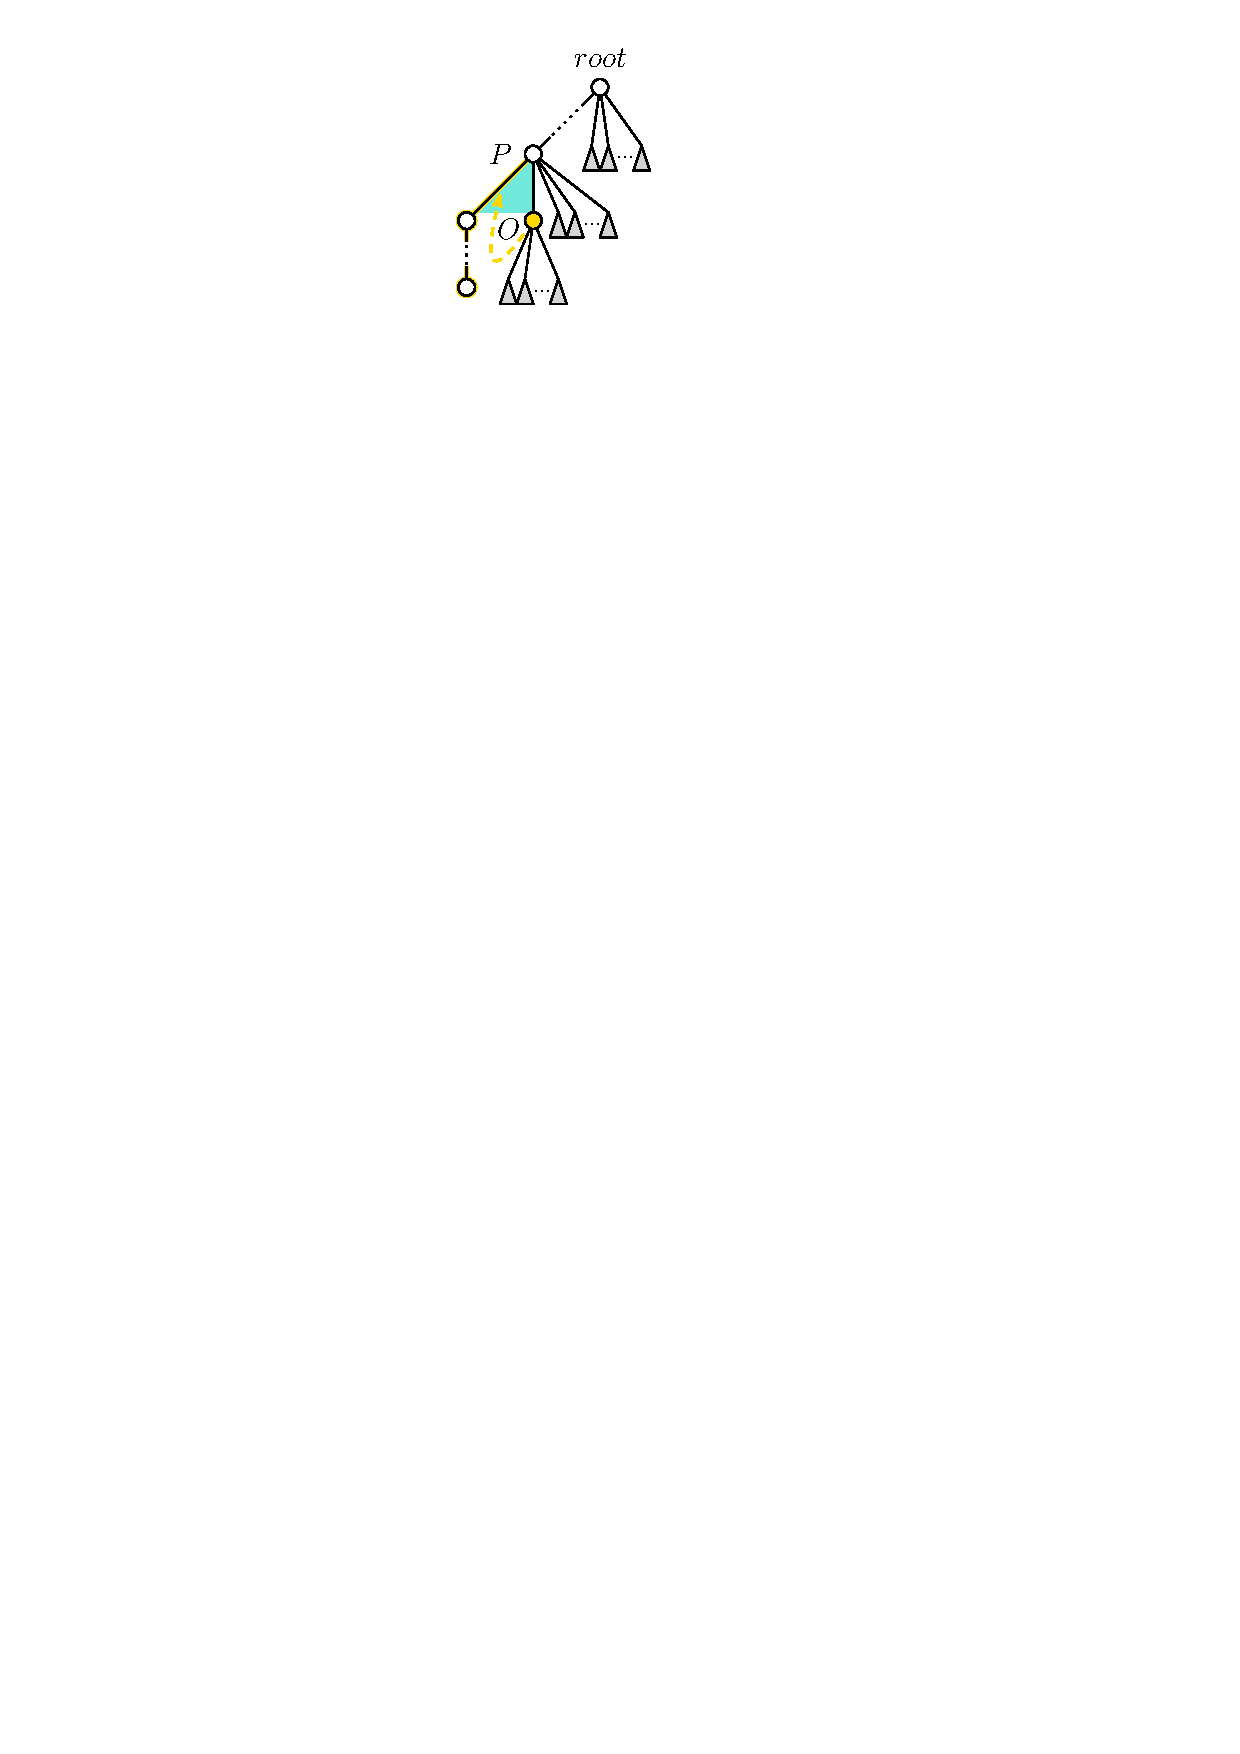
\includegraphics[scale=0.85]{nextTightOr011Before.pdf}
    	    \caption*{Current tree $\tree{T}$ where ${P} = {root}$ or ${O}$ is not a leaf.}
            \label{fig:next1_Before}
        \end{subfigure}
        \hfill
        \begin{subfigure}[t]{.49\textwidth}
    	    \centering
    	    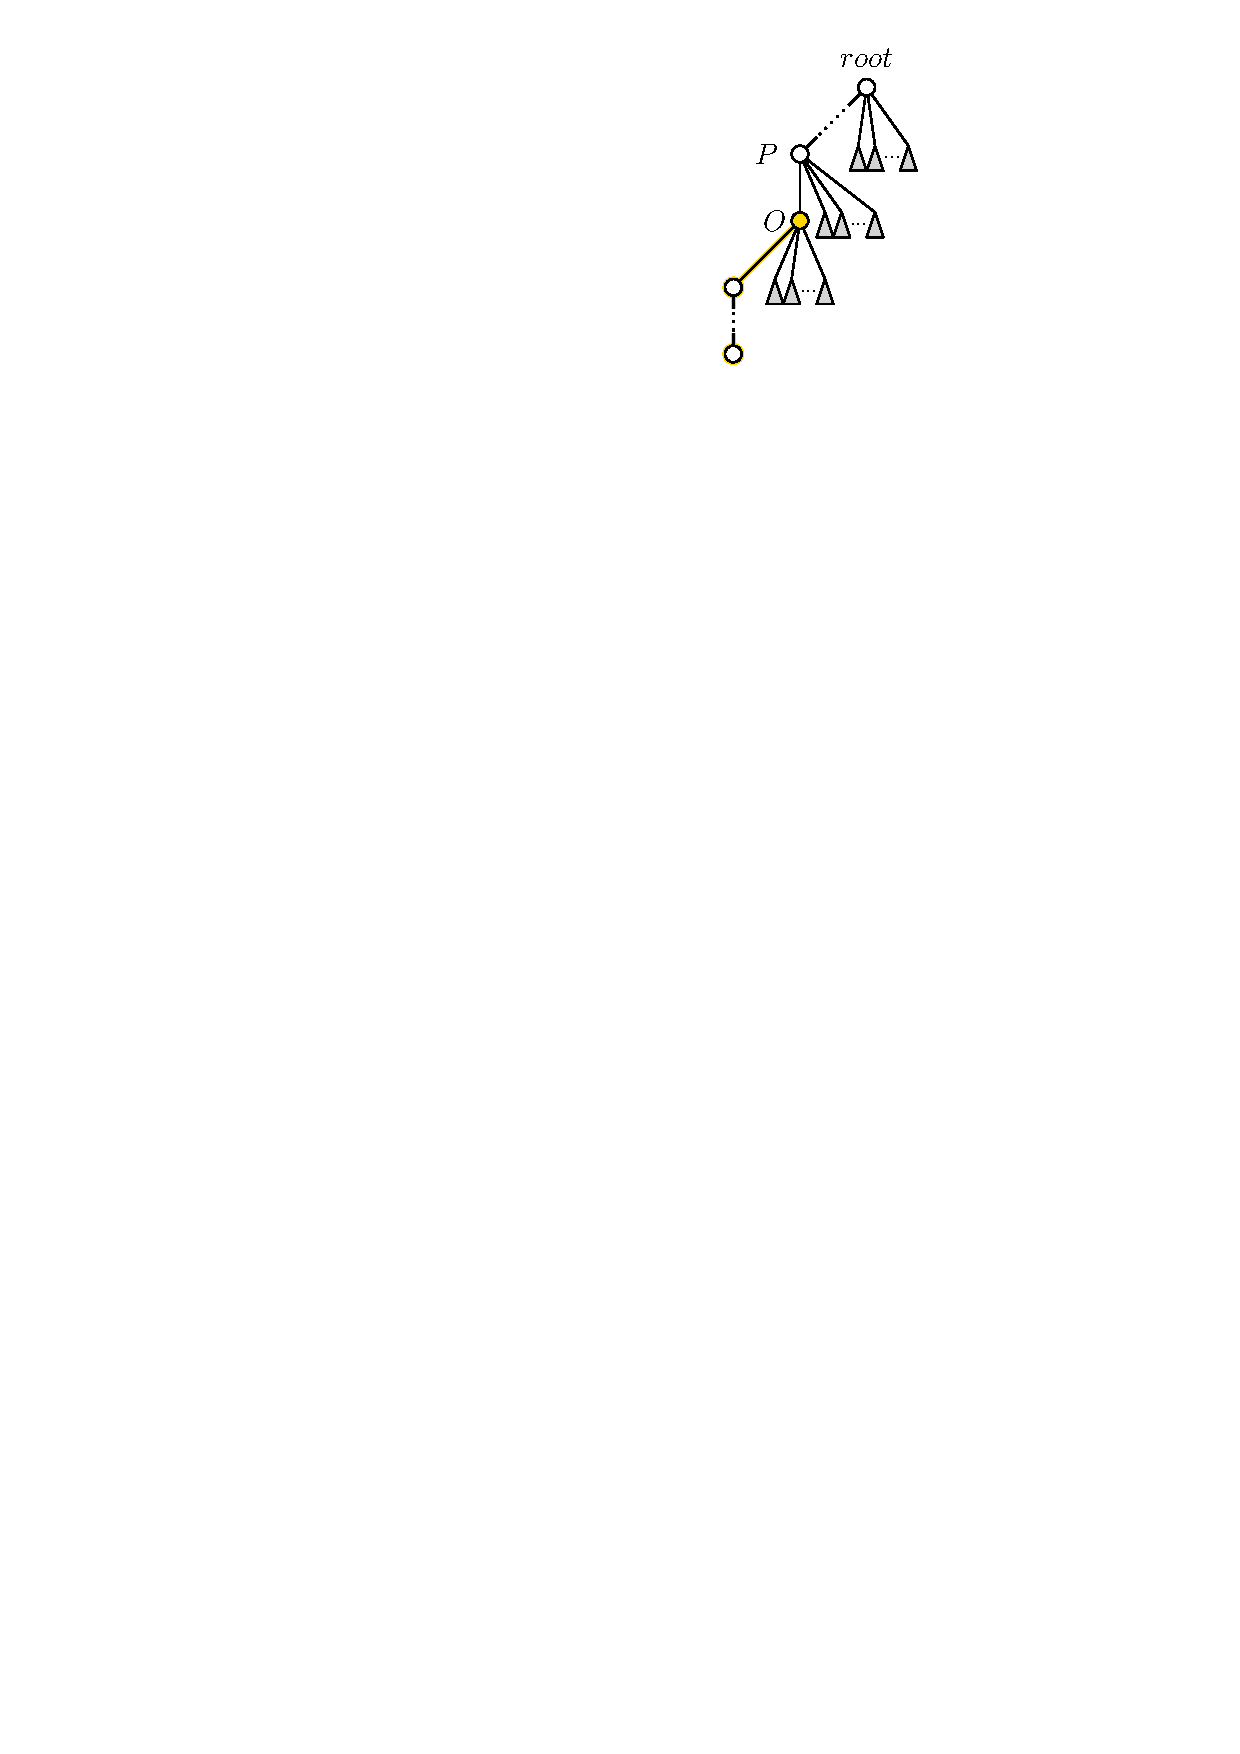
\includegraphics[scale=0.85]{nextTightOr011After.pdf}
    	    \caption*{New tree $\tree{T'}$ is obtained by $\pull[\tree{T}]{{O}}{{P}}$.}
            \label{fig:next1_Intermediate}
        \end{subfigure}
	    \caption{Case \eqref{eq:otree_oneshift}.
	    After the pull, the node ${O}$ is updated to be the new second-child of ${O}$ (if non-null) or the new second-child of ${P}$ (if non-null), or~${null}$.
	    The pull is equivalent to $\pushchild{{O}}{\popchild{{P}}}$.}
        \label{fig:next1}
    \end{subfigure}    

    \vspace{1em}
        
    \begin{subfigure}{.98\textwidth}
        \captionsetup[subfigure]{justification=centering}
        \begin{subfigure}[t]{.32\textwidth}
            \centering
    	    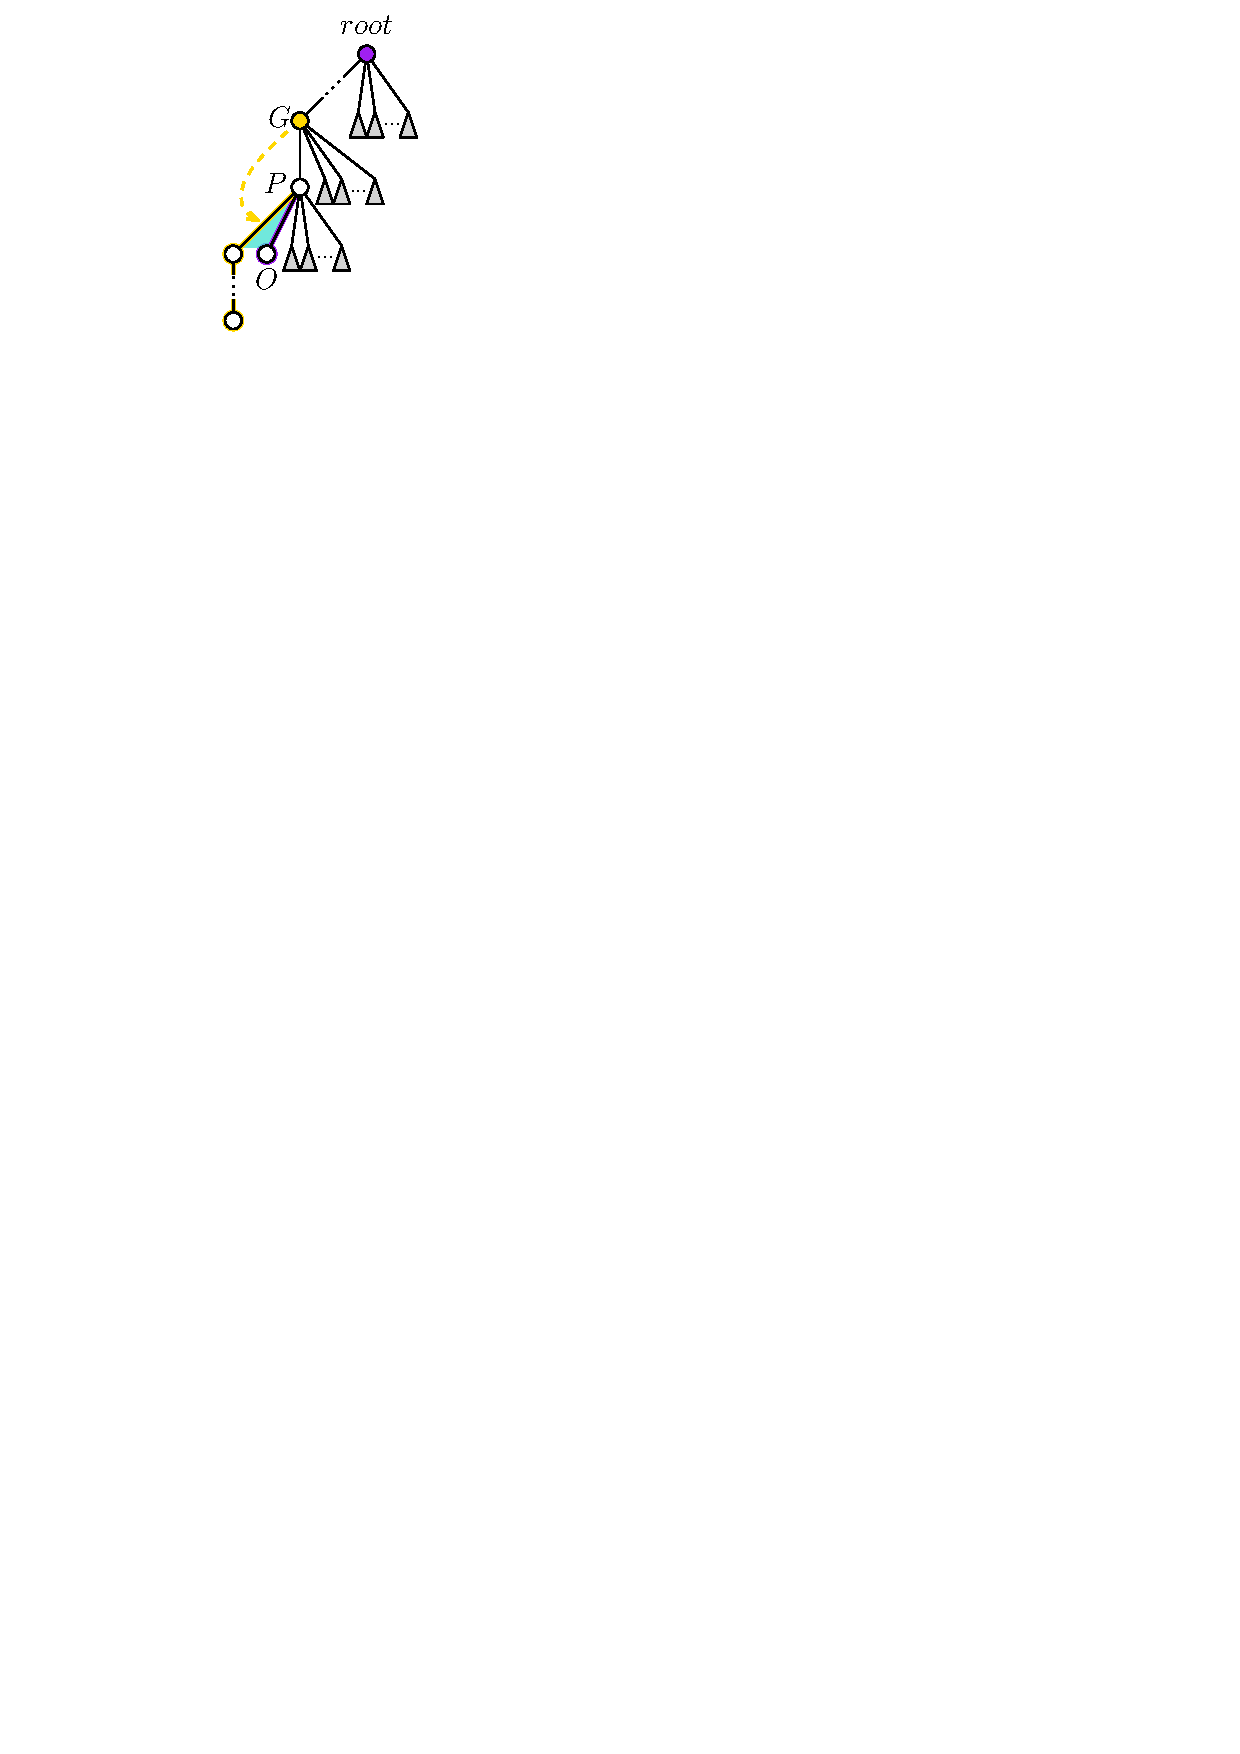
\includegraphics[scale=0.85]{next010Before.pdf}
    	    \caption*{Current tree $\tree{T}$ where ${P} \neq {root}$ and ${O}$ is a leaf.}
            \label{fig:next0_Before}
        \end{subfigure}
        \hfill
        \begin{subfigure}[t]{.32\textwidth}
    	    \centering
    	    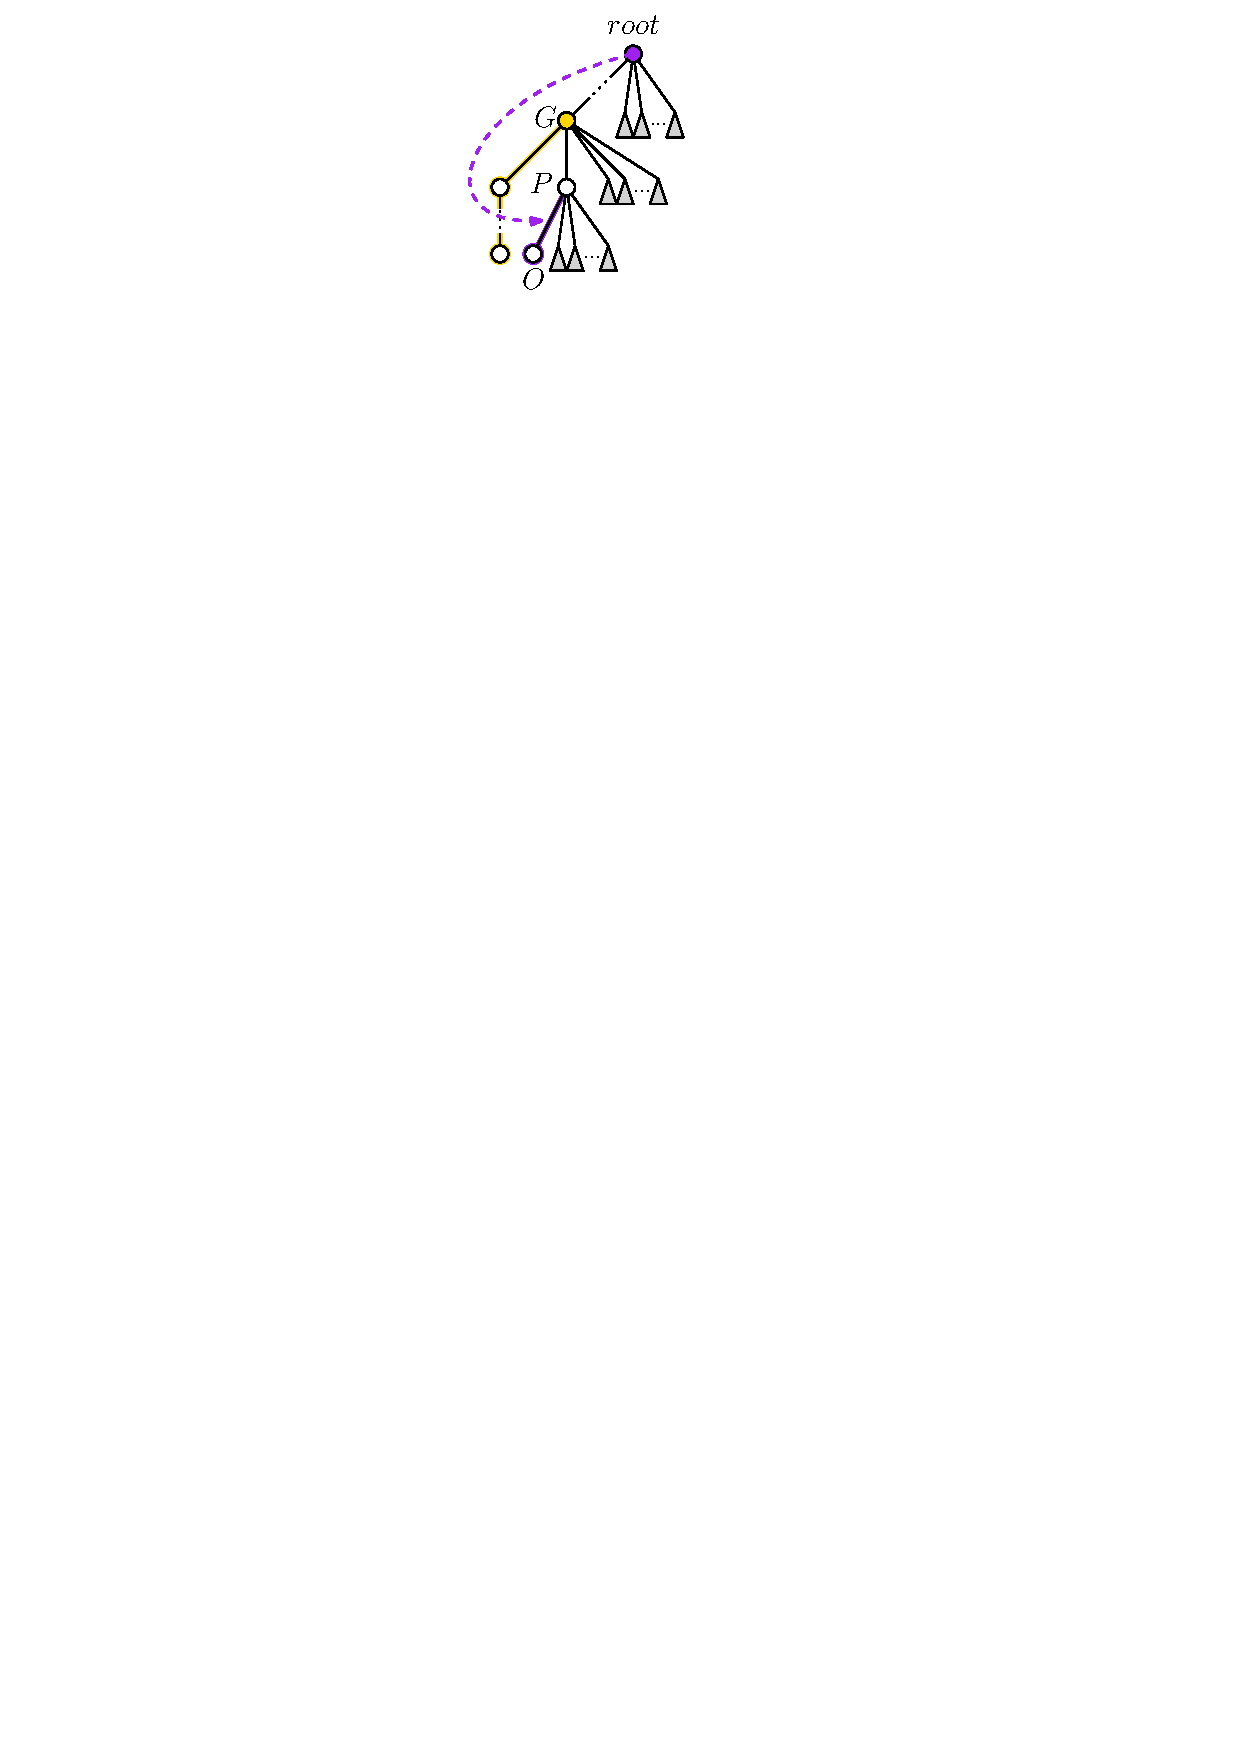
\includegraphics[scale=0.85]{next010Intermediate.pdf}
    	    \caption*{Intermediate tree $\tree{I}$ is obtained by $\pull[\tree{T}]{{G}}{{P}}$.}
            \label{fig:next0_Intermediate}
        \end{subfigure}
        \begin{subfigure}[t]{.32\textwidth}
    	    \centering
    	    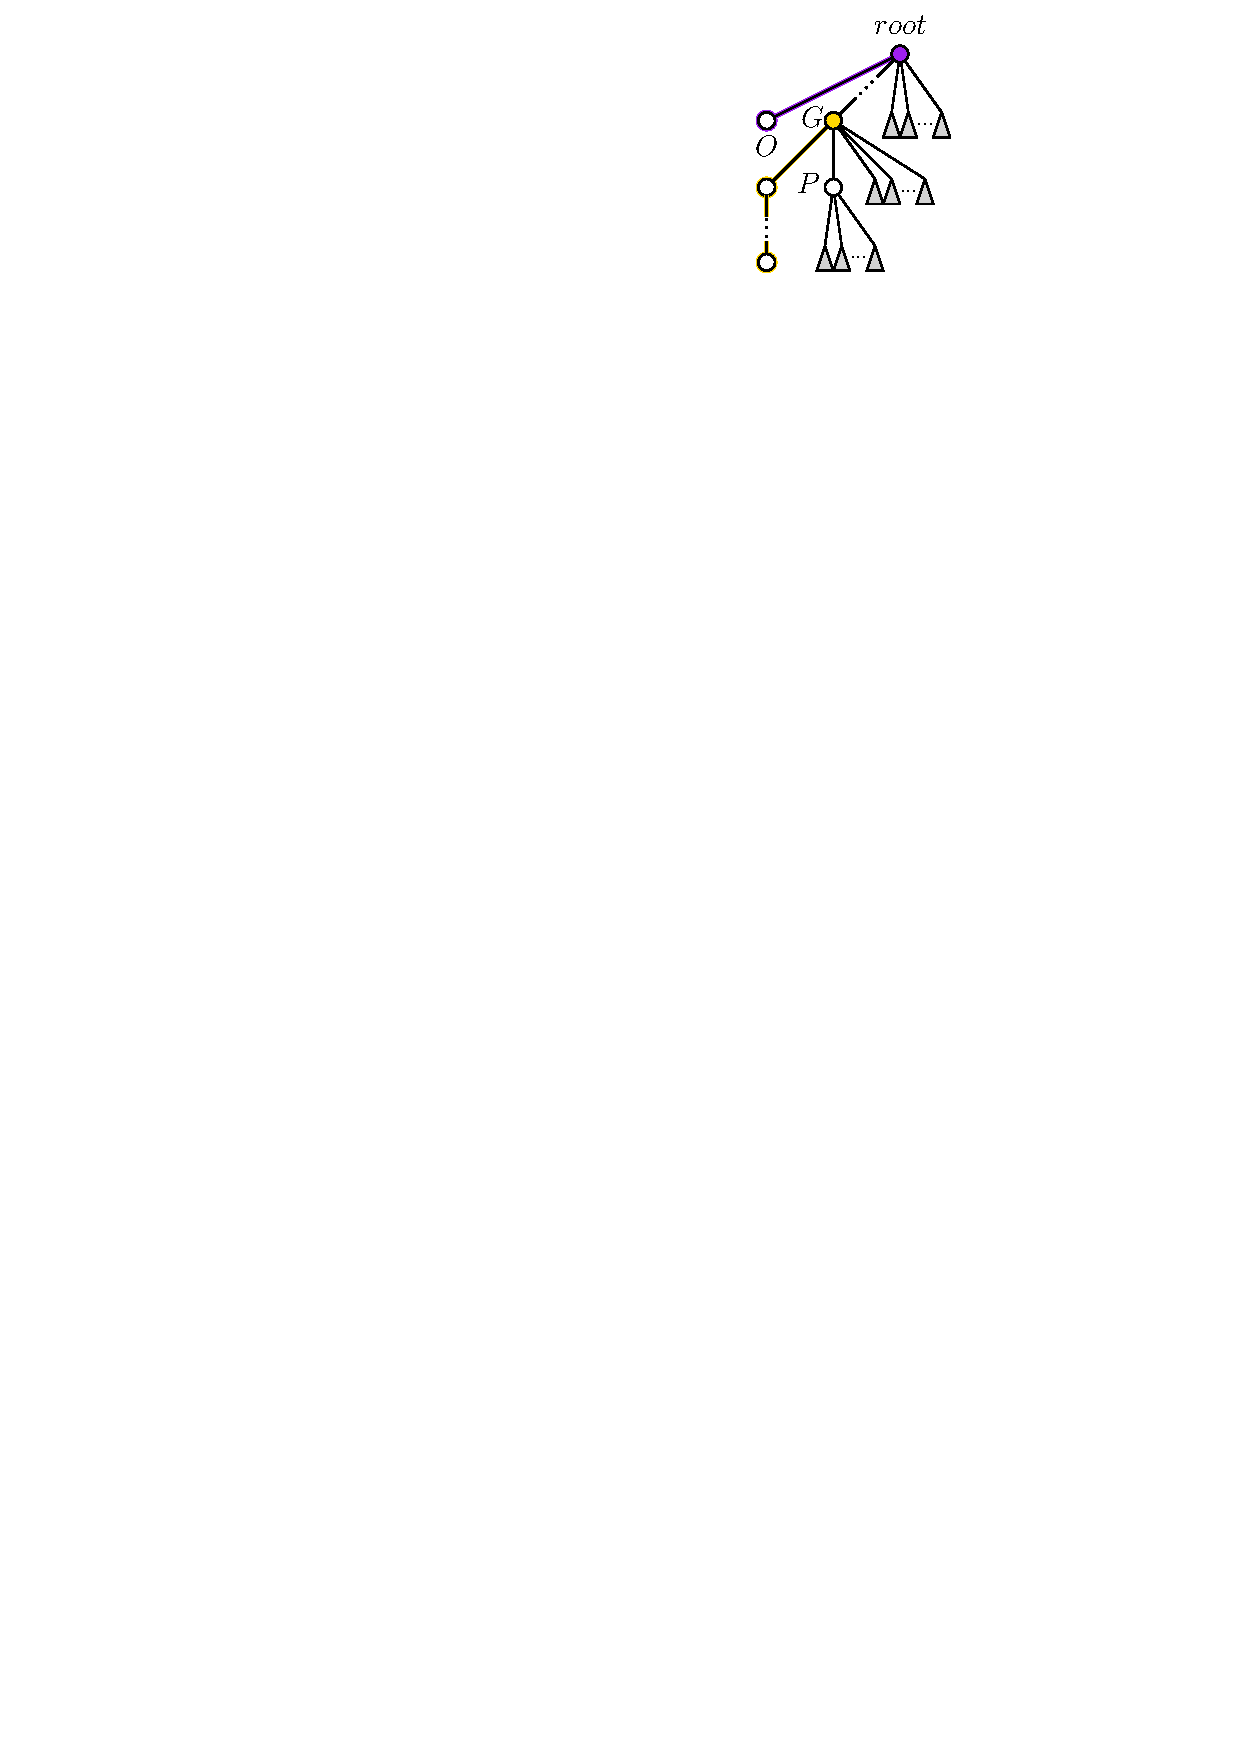
\includegraphics[scale=0.85]{next010After.pdf}
    	    \caption*{New tree $\tree{T'}$ is obtained by $\pull[\tree{I}]{{root}}{{P}}$.}
            \label{fig:next0_After}
        \end{subfigure}
	    \caption{Case \eqref{eq:otree_zeroshift}.
	    After the pull, the node ${O}$ is updated to be the new second-child of ${root}$.
	    The pull operations are equivalent to $\pushchild{{G}}{\popchild{{P}}}$ followed by $\pushchild{{root}}{\popchild{{P}}}$}
        \label{fig:next0}
    \end{subfigure}    
    
    \caption[Our pull Gray code is generated by the two case successor rule in \eqref{eq:otreeRule}.]{Our pull Gray code is generated by the two case successor rule in \eqref{eq:otreeRule}.
    This rule describes how to transform the current ordered tree $\tree{T}$ into the new next ordered tree $\tree{T'}$ using either one or two pulls.
    In these figures, ${O}$ is the first node in a preorder traversal that is not on the path from the root to the leftmost descendent, and ${P}$ is its parent, and ${G}$ is its grandparent (if applicable).
    White circles denote non-null nodes, and grey triangles denote an unspecified number of children and subtrees.
    The pull operations, which are always path-pulls, are highlighted.
    The first pulling node and pulled path are in gold, while the second are in purple.
    The captions also explain how to update the value of ${O}$.}
    \label{fig:next}
\end{figure}


% included from otree-graycode.tex
\begin{figure}
    % Triangles and dashed sections are a work in progress
    \begin{subfigure}[]{.5 \textwidth}
	\begin{center}
	    $1110011100 \implies 1111001100 $

\begin{tikzpicture}[every tree node/.style={draw,circle},sibling distance=10pt, level distance=40pt]
\tikzset{every tree node/.style={minimum width=1.5em,draw,circle}, blank/.style={draw=none}, edge from parent/.style= {draw,edge from parent path={(\tikzparentnode) -- (\tikzchildnode)}}, level distance=1.5cm}
    \Tree[.\node[style={fill=lightyellow}]{G}; [.\node[style={fill=lightpurple}]{P}; [.\node[style={fill=pink}]{L}; [.\node{};  ] ] [.\node[style={fill=lightblue}]{O}; [.{} ] ] [.{} ] ] ] 
\end{tikzpicture}
$\implies$
\begin{tikzpicture}[every tree node/.style={draw,circle},sibling distance=10pt, level distance=40pt]
\tikzset{every tree node/.style={minimum width=1.5em,draw,circle}, blank/.style={draw=none}, edge from parent/.style= {draw,edge from parent path={(\tikzparentnode) -- (\tikzchildnode)}}, level distance=1.5cm}
\Tree[.\node[style={fill=lightyellow}]{G}; [.\node[style={fill=lightpurple}]{P}; [.\node[style={fill=lightblue}]{O}; [.\node[style={fill=pink}]{L}; [.\node{};  ] ] [.{} ] ] [.{} ] ] ] 
\end{tikzpicture}

	\end{center}
	\caption{$O$ has at least 1 child: Case \eqref{eq:otree_oneshift}\\
	$\poppush{O}{P}$ \\
	$L$ becomes $O$'s first child.  The new first branching is between $O$ and $O$'s second child.
	}
	\label{fig:}
    \end{subfigure}
    \begin{subfigure}[]{.49 \textwidth}
	\begin{center}
	    $11111000100100 \implies 10111100010100$

\begin{tikzpicture}[every tree node/.style={draw,circle},sibling distance=10pt, level distance=40pt]
\tikzset{every tree node/.style={minimum width=1.5em,draw,circle}, blank/.style={draw=none}, edge from parent/.style= {draw,edge from parent path={(\tikzparentnode) -- (\tikzchildnode)}}, level distance=1.5cm}
\Tree[.{} [.\node[style={fill=lightyellow}]{G}; [.\node[style={fill=lightpurple}]{P}; [.\node[style={fill=pink}]{L}; [.{} [.{} ] ] ] [.\node[style={fill=lightblue}]{O}; ] ] [.{} ] ] ] 
\end{tikzpicture}
$\implies$
\begin{tikzpicture}[every tree node/.style={draw,circle},sibling distance=10pt, level distance=40pt]
\tikzset{every tree node/.style={minimum width=1.5em,draw,circle}, blank/.style={draw=none}, edge from parent/.style= {draw,edge from parent path={(\tikzparentnode) -- (\tikzchildnode)}}, level distance=1.5cm}
\Tree[.{} [.\node[style={fill=lightblue}]{O}; ] [.\node[style={fill=lightyellow}]{G}; [.\node[style={fill=pink}]{L}; [.{} [.{} ] ] ] [.\node[style={fill=lightpurple}]{P}; ] [.{} ] ] ] 
\end{tikzpicture}

	\end{center}
	\caption{ $P \ne root$, $O$ has no children: Case \eqref{eq:otree_zeroshift}\\
	$\poppush{G}{P};\poppush{root}{P}$ \\
	$L$ becomes $G$'s first child; $O$ becomes the first child of $root$.  The new first branching is between the root and the root's second child.\\
	% test
	}
	\label{fig:}
    \end{subfigure}

\bigskip

    \begin{subfigure}[]{.5 \textwidth}
	\begin{center}
	    $1110001010 \implies 1111000010$

%1110001010
\begin{tikzpicture}[every tree node/.style={draw,circle},sibling distance=10pt, level distance=40pt]
\tikzset{every tree node/.style={minimum width=1.5em,draw,circle}, blank/.style={draw=none}, edge from parent/.style= {draw,edge from parent path={(\tikzparentnode) -- (\tikzchildnode)}}, level distance=1.5cm}
\Tree[.\node[style={fill=lightpurple}]{P}; [.\node[style={fill=pink}]{L}; [.{} [.{} ] ] ] [.\node[style={fill=lightblue}]{O}; ] [.{} ] ] 
\end{tikzpicture}
$\implies$
%1111000010
\begin{tikzpicture}[every tree node/.style={draw,circle},sibling distance=10pt, level distance=40pt]
\tikzset{every tree node/.style={minimum width=1.5em,draw,circle}, blank/.style={draw=none}, edge from parent/.style= {draw,edge from parent path={(\tikzparentnode) -- (\tikzchildnode)}}, level distance=1.5cm}
\Tree[.\node[style={fill=lightpurple}]{P}; [.\node[style={fill=lightblue}]{O}; [.\node[style={fill=pink}]{L}; [.{} [.{} ] ] ] ] [.{} ] ] 
\end{tikzpicture}

	\end{center}
	\caption{$O$ has no children, $P = root$: Case \eqref{eq:otree_oneshift}\\
	$\poppush{O}{P}$ \\
	    $L$ becomes $O$'s first child. The new first branching is between $P$ and $P$'s second child.
	}
	\label{fig:}
    \end{subfigure}
    \begin{subfigure}[]{.49 \textwidth}
	\begin{center}
	    $1111100000\implies 1011110000$

\begin{tikzpicture}[every tree node/.style={draw,circle},sibling distance=10pt, level distance=40pt]
    \tikzset{every tree node/.style={minimum width=1.5em,draw,circle}, blank/.style={draw=none}, dotted/.style={draw=gray,dashed,thick},edge from parent/.style= {draw,edge from parent path={(\tikzparentnode) -- (\tikzchildnode)}}, level distance=1.5cm}
\Tree[.{} [.\node{}; [.{} [.\node[style={fill=lightyellow}]{G}; [.\node[style={fill=lightpurple}]{P}; [.\node[style={fill=lightblue}]{O}; ] ] ] ] ] ] 
\end{tikzpicture}
$\implies$
\begin{tikzpicture}[every tree node/.style={draw,circle},sibling distance=10pt, level distance=40pt]
\tikzset{every tree node/.style={minimum width=1.5em,draw,circle}, blank/.style={draw=none}, dotted/.style={draw=gray,dashed,thick},edge from parent/.style= {draw,edge from parent path={(\tikzparentnode) -- (\tikzchildnode)}}, level distance=1.5cm}
\Tree[.{} [.\node[style={fill=lightblue}]{O}; ] [.\node{};  [.{} [.\node[style={fill=lightyellow}]{G}; [.\node[style={fill=lightpurple}]{P}; ] ] ] ] ] 
\end{tikzpicture}

	\end{center}
	\caption{$\tree{T}$ has no first branching: Case \eqref{eq:otree_noo_cyclic} \\
	$\poppush{root}{P}$ \\
	O becomes the first child of the root \\
	The new first branching is between the root and the root's second child.
	}
	\label{fig:}
    \end{subfigure}
    % TODO NEW: more robust caption
    \caption{Illustrating pull shifts on specific trees.
    %In these diagrams, $O$ is the child of the first branching in $\tree{T}$ or $\tree{T}$'s leaf if T has no first branching.  $P$ is $O$'s parent, $G$ is $P$'s parent (if it exists), and $L$ is $O$'s left sibling.
    }
    \label{fig:otreeruledemo}

\end{figure}



\section{Proof of Correctness} \label{sec:otree-proof}

This section will prove that the successsor rule does in fact in \eqref{eq:otreeRule} generates all ordered trees with $n$ nodes. 
\subsection{Definitions and Remarks}

Let $\tree{T}$ be an ordered tree with $n+1$ nodes listed in preorder as $t_0,t_1,...,t_n$.  Note that $t_0$ is the root of $\tree{T}$. We define the \emph{left-down path} of $\tree{T}$, $\leftdown{\tree{T}},$ to be the unique path between $\tree{T}$'s root and $\tree{T}$'s leftost leaf.
Let $D=\dyck{T}$.  Let $x$ be the index of the first $1$ following a $0$ in $D$, mirroring section \ref{sec:coolDyck}.  Let $s$ be the number of consecutive ones to start D and let $z$ be the number of consecutive zeroes starting at $d_{s+1}$.  Note that $z=(x-s-1)$; $d_{x}=1$.  Let $\oneindex{D}{i}=$ be the index of the $i\thh{}$ one in $D$.
The following remarks can be derived from from the above definitions and the bijection between Dyck words and ordered trees given in given in \ref{subsec:otree-dyck-bij}.


\begin{remark} $\depth{O}=s-z+1$ \label{re:o_depth_formula}
    % \bigskip
\end{remark} 
\begin{proof}


    $t_s$ is the last node in the $\leftdown{\tree{T}}$, as the left-down path has $s+1$ nodes starting at $t_0$. $t_s$ has depth s, as it is exactly s steps from the root.  Note that $O=t_{s+1}$.  The number of zeroes between $t_s$ and $t_{s+1}$ is the number of zeroes between the $s\thh$ and $(s+1)^{\underline{st}}$ ones in $D_i$.  

\end{proof} 
\begin{remark}O corresponds to $D_x$%, i.e. $\oneindex{D}{s+1}=x$
\end{remark}
\begin{proof}
    Recall that $O$ is the first branching of $\tree{T}$ and the first second child visited in a preorder traversal of $\tree{T}$.

    Recall that in the bijection between ordered trees and Dyck words given in \ref{subsec:otree-dyck-bij} that each 1 in D corresponds to a step down and each 0 corresponds to a step up.  A second child in a preorder traversal of an ordered tree must be equal to the 
    %Consequently, $\leftdown{\tree{T}}$ corresponds to the ``all-one" prefix of D.  In other words, $\leftdown{\tree{T}}=t_0,t_1,...t_{s}$ such that $i=0$ or $D_i=1$. Note that $t_{s+1}$ is therefore the first node in a preorder traversal of T such that $D_{\oneindex{D}{s+1}}=1$ and $D_{\oneindex{D}{s+1}-1}=0$.  O is therefore also the first node in a preorder traversal of T such that $t_{s+1} \notin \leftdown{\tree{T}}$.  Therfore, $\oneindex{D}{s+1}=x$, i.e., $t_{s+1}=O$ corresponds to the 1 in the leftmost 01 substring of D.

\end{proof}
\begin{remark} Every non-leaf node below P in $\leftdown{\tree{T}}$ has exactly 1 child.  \label{rem:left-is-path}
\end{remark}

\begin{proof}
    Suppose by way of contradiction that a node below P in $\leftdown{\tree{T}}$ had a second child. That child would not be in $\leftdown{\tree{T}}$ and would be be traversed before O in preorder. O was specified to be the first node in a preorder traversal of T that is not in $\leftdown{\tree{T}}$, which generates a contradiction.

\end{proof}

\begin{remark} \label{re:L_sz1}
    $L$ corresponds to $D_{s-z+1}$ %, i.e. $\oneindex{D}{s-z+1}=s-z+1$
\end{remark}
\begin{proof}

    $\depth{L}=\depth{O}=s-z-1$ since L and O are siblings. Therefore, L must be $s-z-1$ steps down from the root $\implies$ $L$ is the $s-j-1$th node in a preorder traversal of T $\implies$ T corresponds to $D_{s-z-1}$.


\end{proof}


% \end{enumerate}

% Ruskey and Williams proved that, given a Dyck word of order n, \eqref{eq:prefixDyck} iteratively generates all Dyck words of order n.  This proof will use the bijection between Dyck words of order $n$ and ordered trees with $n+1$ nodes to show that that \eqref{eq:otreeRule} generates all ordered trees with a given number of nodes.  



% The  has many useful properties for proving the correspondence between \eqref{eq:prefixDyck} and \eqref{eq:otreeRule}.


% \begin{itemize}
%     % \item Let $\otree{D}$ and $\dyck{T}$ be functions that convert a Dyck word to an ordered tree and an ordered tree to a Dyck word respectively via the process outlined in 
%     % \item Let $\depth{t_i}=$ length of the path between root and $t_i$. $\depth{root}=0$
%     \item 
% \end{itemize}



% the following remarks can be derived from the bijection between ordered trees and Dyck words. 
% Given an ordered tree $\tree{T}$, its preorder listing $t_0,t_1,...t_n$, and its corresponding order $n$ Dyck word $D$
\begin{remark}
    The $i\thh$ non-root node in a preorder listing of $\tree{T}$ corresponds to the $i\thh$ one in $D$.

    % Equivalently, $t_i$ corresponds to the $\oneindex{D}{i}$ one in D for $1 \le i \le n$
\end{remark}
\begin{proof}
    Recall the method of constructing an ordered tree from a Dyck word.  Each one in D creates a new node; zeroes in D do not create nodes.  Generating an ordered tree from a Dyck word generates the nodes of the tree in preorder.  Thus, $t_i$ corresponds to the $i$th one in D for $1 \le i \le n$.
\end{proof}

\begin{remark} The difference in depths between nodes $t_i$ and $t_{i-1}$ is equal to one minus the number of zeroes between the $(i-1)^{\underline{st}}$ and $i\thh$ and  ones in $D$


\end{remark}
\begin{proof}

    This remark can be stated formally as 

    \begin{equation} \label{eq:depthformula} 
    	\depth{t_i} - \depth{t_{i-1}}=1-(\oneindex{D}{i}-\oneindex{D}{i-1} - 1) 
    \end{equation}
    

    % or equivalently, 

    % \begin{equation} \label{eq:indexformula} 
    % 	\oneindex{D}{i} = \oneindex{D}{i-1} + \depth{t_{i-1}} - \depth{t_i} + 2
    % \end{equation}
    

    Note that $(\oneindex{D}{i}-\oneindex{D}{i-1}-1)$ is equal to the number of zeroes between the $i\thh$ and $(i-1)^{\underline{st}}$ ones in D.  % Therefore, this rule can be informally described as follows:

    % The depth of $t_i$ is the depth of $t_{i-1}$ plus 1 minus the number of zeroes between the $(i-1)\thh$ and $i\thh$ ones in D

    % The number of zeroes between the $i\thh$ and $(i-1)\thh$ ones in $D$ is equal to one plus the depth  $\depth{t_i}$ minus $\depth{t_{i-1}}$

    This follows naturally from the bijection between Dyck words and ordered trees.  Each zero corresponds to a step up in the tree before adding the next child.  

    If there are zero zeroes between the $i\thh$  and $(i-1)^{\underline{st}}$ ones in D, $t_i$ is a child of $t_{i-1}$; $\depth{t_i}=\depth{t_{i-1}}+1$

    If there is one zero between the $i\thh$  and $(i-1)^{\underline{st}}$ ones in D, $t_i$ is a child of $t_{i-1}$'s parent; $\depth{t_i}=\depth{t_{i-1}}+1$.  

    Each subsequent zero between $t_{i-1}$ and $t_i$ decreases $\depth{t_{i}}$ by one.  Thus, the depth of $t_i$ is the depth of $t_{i-1}$ plus 1 minus the number of zeroes between $t_{i-1}$ and $t_{i}$.
\end{proof}
% \bigskip


\begin{remark}A preorder listing of $\depth{t_i} $ for each $ t_i \in T$ can be used to construct a Dyck word. \label{re:construct_dyck}

\end{remark} 
\begin{proof}
    % This follows from Remark \ref{re:depthformula}, as it implies that for any $i,i+1 \le n$, $\oneindex{D}-\oneindex{$ 

    Let $\tree{T}=t_0,t_1,...t_n$ be a preorder traversal of T.  Note that $t_0$ is the root of $\tree{T}$

    Construct D as follows: 

    \begin{itemize}
	% \item skip $t_0$
	\item Let $D=\epsilon$ % clear that this is empty string?
	\item For each $t_i$, $1\le i \le n$
	    \begin{itemize}
		\item Append a 1 to $D$
		\item Append $1-\depth{t_{i}}+\depth{t_{i-1}}$ zeroes to D.
	    \end{itemize}
	\item Append $\depth{t_{n}}$ zeroes to D. 
    \end{itemize}
\end{proof} 

% \section{ $\overleftarrow{\mathsf{coolCat}} \iff \mathsf{nextree}$ }
\subsection{Correspondence between coolCat and nextree}
Recall that the successor rule $\coolCat{D}$ generates all Dyck words.  Therefore,  to prove that $\nextTree{T}$ generates all ordered trees with $|T|$ nodes, it is sufficient to show that, given an arbitrary ordered tree T and its corresponding Dyck word D, $\nextTree{T}$ behaves the same on T as $\coolCat{D}$ does on D. More precisely, we aim to prove the following: 



\begin{theorem}
    Given an ordered tree T, $\nextTree{T}=\otree{\coolCat{\dyck{T}}}$
\end{theorem}

\begin{proof}




% First, consider the node O in the specification of the $\nextTree{T}$ algorithm.  




$\coolCat{D}$ and $\nextTree{T}$ are each broken down into 3 cases in equations \eqref{eq:prefixDyck} and \eqref{eq:otreeRule} respectively. 

For convenience, equations \eqref{eq:expandedOtree} and \eqref{eq:expandedDyck}  give the expanded restatemtents of the successor rules for $\nextTree{T}$ and $\coolCat{D}$ to facilitate comparisons between the two.  %Recall that $s$ is the number of consecutive ones at the start of $D$.

\begin{subnumcases}{\nextTree{T} = \label{eq:expandedOtree}}
    \poppush{P}{root}  & $\leftdown{\tree{T}}=\tree{T}$ \label{eq:ex_otree_n}\\
    \poppush{P}{O}  & if O has at least 1 child \label{eq:ex_otree_k1_1} \\
    \poppush{P}{G};\poppush{P}{root} & if $P \ne root $ and O has no children \label{eq:ex_otree_k1_0} \\
    \poppush{P}{O}  & if O has no children and $P=root$ \label{eq:ex_otree_k}
\end{subnumcases}

\begin{subnumcases}{\coolCat{D} = \label{eq:expandedDyck}}
    \preshift{D}{2n} & \text{if $D$ has no $01$ substring} \label{eq:expandedDyck_n}\\
    \preshift{D}{x+1} & $D_{x+1}=1$ \label{eq:expandedDyck_k1_1}\\
    \preshift{D}{x+1} & $D_{x+1}=0$ and $s>\frac{x-1}{2}$ \label{eq:expandedDyck_k1_0}\\
    \preshift{D}{x} & $D_{x+1}=0$ and $s=\frac{x-1}{2}$ \label{eq:expandedDyck_k}
\end{subnumcases}


% \footnote{important: 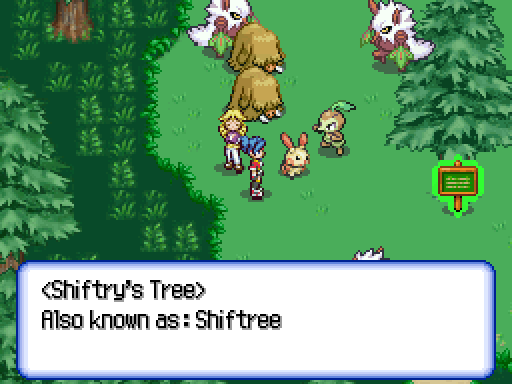
\includegraphics[width=.3\textwidth]{shiftree}} 


We will show the following equivalences:

\begin{itemize}
    \item \eqref{eq:ex_otree_n} corresponds to \eqref{eq:expandedDyck_n}
    \item \eqref{eq:ex_otree_k1_1} corresponds to \eqref{eq:expandedDyck_k1_1}
    \item \eqref{eq:ex_otree_k1_0} corresponds to \eqref{eq:expandedDyck_k1_0}
    \item \eqref{eq:ex_otree_k} corresponds to \eqref{eq:expandedDyck_k}
\end{itemize}

To accomplish this, we will first prove a few auxillary lemmas to be used to show equivalency between cases. 

Let $D=\dyck{T}$, $s$ be the number of consecutive ones to start D, and $z$ be the number of consecutive zeroes starting at $d_{s+1}$.  Note that $z=(x-s-1)$; $d_{x}=1$
% \begin{itemize}
\begin{lemma} \label{le:final_case_equivalence}

    $D$ has no 01 substring $\iff$ $\leftdown{\tree{T}}=\tree{T}$
\end{lemma}
\begin{proof}


    If $D$ has no $01$ substring, $D=1^n0^n$, and T is $n+1$ nodes where $t_0$ is the root and each $t_i$ for $1\le i \le n$ is a child of $t_{i-1}$  In this case, $\tree{T}$ is a single path of $n+1$ nodes, and the left-down path of T is the entire tree.
\end{proof}
\begin{lemma} \label{le:no_children_equivalence}
    $D_{x+1} = 0 \iff O$ has no children
\end{lemma}
\begin{proof}

    This follows logically from the bijection between Dyck words and ordered trees.  $D_x$ corresponds to O.  If $D_{x+1}=0$, an ``upward" step is taken after O and consequently the next node after O cannot be a child of O.  Since the ones in $D$ give the nodes of T in preorder, O must have no children.

    Informally, once you go ``up" from O, the bijection between Dyck words and ordered trees gives no way to go ``back down" to give O an additional child.
\end{proof}
\begin{lemma} \label{le:tight_case_equivalence}
    $P=root \iff s=z=\frac{x-1}{2}$.
\end{lemma}
\begin{proof}

    First, note that $P=root$ simply means that O is a child of the root.  O is a child of the root $\iff \depth{O}=1$.  Additionally, note that $s+z=x-1$

    As shown in remark \ref{re:o_depth_formula}, $\depth{O}=s-z+1$. Therefore, $P=root \iff s=z=\frac{x-1}{2}$
    i.e. the first $x-1$ symbols of D are $\frac{x-1}{2}$ ones followed by $\frac{x-1}{2}$ zeroes. 

    % This equivalence can can be rewriten as follows: 

    % $s=x-s-1$

    % $2s=x-1$

    % $s=\frac{x-1}{2}$



\end{proof}
% \begin{enumerate}
\begin{lemma}
    \eqref{eq:ex_otree_n} corresponds to \eqref{eq:expandedDyck_n}
\end{lemma}
\begin{proof}

    Let $D=\dyck{T}$

    Per lemma \ref{le:final_case_equivalence} $D$ has no 01 substring $\iff$ $\leftdown{\tree{T}}=\tree{T}$.  

    Thus, $\nextTree{T}$ executes case \eqref{eq:ex_otree_n} if and only if $\coolCat{D}$ executes case  \eqref{eq:expandedDyck_n}

    Note that since $D$ has no $01$ substring, $D=1^n0^n$. 

    Additionally, since $\leftdown{\tree{T}}=\tree{T}$, T can be specified as follows.

    $\tree{T}=$
    \begin{center}
	\begin{tabular}{ |c|c|c|c|c|c|c|c|c|c|c| } 
	    \hline

	    $node$ & $t_0$ & $t_1$  & $t_2$ & $\dots$ & $t_{n-1}$&$F=t_s=t_n$  \\
	    \hline
	    $depth$ & $0$ & $1$ & $2$ & $\dots$ & $n-1$ & $n$ \\
	    \hline
	    $Dyck$ &  &  \multicolumn{5}{|c|}{$1^n0^n$} \\
	    \hline
	\end{tabular}
    \end{center}

    The third row of this table illustrates the construction of $\dyck{T}$ via the process specified in remark \ref{re:construct_dyck}.

    Shifting $F$ to be the first child of the root changes $\depth{F}$ to 1 and does not affect the depth of any other nodes.  Thus, if $\tree{T}'=\nextTree{T}$, 


    $\tree{T}=$
    \begin{center}
	\begin{tabular}{ |c|c|c|c|c|c|c|c|c|c|c| } 
	    \hline

	    $node$ & $t_0$ & $F=t_s=t_n$ & $t_1$  & $t_2$ & $\dots$ & $t_{n-1}$  \\
	    \hline
	    $depth$ & $0$ & $1$ & $1$ & $2$ & $\dots$ & $n-1$ \\
	    \hline
	    $Dyck$ &  &  1 &  \multicolumn{4}{|c|}{$01^{n-1}0^{n-1}$} \\
	    \hline
	\end{tabular}
    \end{center}

    Recall that $\coolCat{D}=\preshift{D}{2n}$ if D has no 01 substring. $D_{2n}=0$, and therefore 

    $\coolCat{D}=101^{n-1}0^{n-1}$
     
     Note that this is exactly the Dyck word constructed from $\tree{T}'$.  Therefore, if D has no 01 substring or $\leftdown{\tree{T}}=\tree{T}$, 

     $\otree{\coolCat{D}}=\nextTree{T}$

\end{proof}
\begin{lemma}
    \eqref{eq:ex_otree_k1_0} corresponds to \eqref{eq:expandedDyck_k1_0}
\end{lemma}
\begin{proof}
    Let $D=\dyck{T}$

    % \begin{itemize}
    Per lemma \ref{le:tight_case_equivalence} $P=root \iff D$ starts with exactly $\frac{x-1}{2}$ ones.  

    It was also previously shown that $D_{x+1}=0 \iff O$ has no children.  
    Thus, $\nextTree{T}$ executes case \eqref{eq:otree_zeroshift} 
    if and only if $\coolCat{D}$ executes case   \eqref{eq:expandedDyck_k1_0}

    \bigskip

    We now show that the execution of \eqref{eq:otree_zeroshift} is equivalent to the execution of \eqref{eq:expandedDyck_k1_0} given case a.
    Given $\dyck{T}=D=1^s0^{z}10d_{x+2}d_{x+3}...d_{2n}$, we aim to show that 

    $\dyck{\nextTree{T}}=\coolCat{\dyck{T}}$
    \bigskip

    Note that in this case $\nextTree{T}$ can be obtained by performing $\poppush{P}{G};\poppush{P}{root}$. 

	    Let $\tree{T}'=\poppush[T]{P}{G}$; $\tree{T}''=\poppush[T']{P}{root}$

	    Note that $\nextTree{T}=\tree{T}''$

    Since $P \ne root$, we know that G, the parent of P, exists. 
    Thus, we can assume that $G,P,L \in \leftdown{\tree{T}}$.  T can therefore be specified as follows: 



    % this should be a little lemma
    % $\tree{T}'$ shifts T so that L becomes the first child of G.  Note that L must have exactly 1 child: otherwise L's second child would be traversed earlier in a preorder traversal than O.  The same logic holds for each subtree of L: Each of L's non-leaf descendents must have exactly one child, as otherwise O would not be the first node in a preorder traversal of T not in $\leftdown{\tree{T}}$.

    \bigskip
    \bigskip

	    $\tree{T}=$
    \begin{center}
	\begin{tabular}{ |c|c|c|c|c|c|c|c|c|c|c| } 
	    \hline

	    $node$ & $t_0$ & $t_1$ & $\dots$ & $G=t_{s-z-1}$ & $P=t_{s-z}$ & $L=t_{s-z+1}$ & $\dots$ & $F=t_s$ & $O=t_{s+1}$ & $\dots$ \\
	    \hline
	    $depth$ & $0$ & $1$ & $\dots$ & $(s-z-1)$ & $(s-z)$ & $(s-z+1)$ & $\dots$ & $s$  & $(s-z+1)$ & $\dots$\\
	    \hline
	    $Dyck$ &  &  \multicolumn{7}{|c|}{$1^s$} &  $0^{z}1$   & $0\dots$\\
	    \hline
	\end{tabular}
    \end{center}
    % Note that $|\leftdown{T'}|=s+1$; as it is nodes $t_0$ through $F$

    Furthermore, recall that L (and all other non-leaf nodes $\in \leftdown{\tree{T}}$ must have exactly one child.  Therefore, every node below L in $\leftdown{\tree{T}}$ has its depth reduced by one; no other nodes have their depth affected by this shift. Therefore, T' can be written as follows:

    \bigskip


	    $\tree{T}'=$
    \begin{center}
	\begin{tabular}{ |c|c|c|c|c|c|c|c|c|c|c| } 
	    \hline

	    $node$ & $t_0$ & $t_1$ & $\dots$ & $G=t_{s-z-1}$ & $L=t_{s-z+1}$ & $\dots$ & $F=t_s$ & $P=t_{s-z}$ & $O=t_{s+1}$ & $\dots$ \\
	    \hline
	    $depth$ & $0$ & $1$ & $\dots$ & $(s-z-1)$ & $(s-z)$ & $\dots$ & $s-1$ & $(s-z)$  & $(s-z+1)$ & $\dots$\\
	    \hline
	    $Dyck$ &  &  \multicolumn{6}{|c|}{$1^{s-1}$} &  $0^{z}1$   & $1$ & $0\dots$\\
	    \hline
	\end{tabular}
    \end{center}

    Since L is now G's first child, P changes from being G's first child to G's second child.  P is therefore removed from the left-down path of $\tree{T}'$, thereby making P the first node in a preorder traversal of $\tree{T}'$ that is not in the left-down path of $\tree{T}'$.  
    Therefore, $|\leftdown{T'}|=s$; $O'=P$. % TODO: check this

    % Note in the case where $z=1$, $L=F=t_s$; i.e. L is the leaf of the left-down path of T.

    Recovering a Dyck word from $\tree{T}'$, we obtain 

    D'=$1^{s-1}0^z110d_{x+2}d_{x+3},\dots,d_{2n}$


    Next, we use $\poppush[T']{P}{root}$
 to obtain $\tree{T}'' = \nextTree{T}$

    $\poppush[T']{P}{root}$
 shifts O to become the first child of the root. Note that we know that O has no children. Consequently, no nodes other than O have their depth affected by this shift. Thus, 

    \bigskip
    \bigskip


    % TODO: tm+2 dots, here and other tables
    $\tree{T}''=$
    \begin{center}
	\begin{tabular}{ |c|c|c|c|c|c|c|c|c|c|c|c| } 
	    \hline

	    $node$ & $t_0$ & $O=t_{s+1}$ & $t_1$ & $t_2$ & $\dots$ & $G=t_{s-z-1}$ & $L=t_{s-z+1}$ & $\dots$ & $F=t_s$ & $P=t_{s-z}$ & $\dots$ \\
	    \hline
	    $depth$ & $0$ & $1$ & $1$ & $2$ &$\dots$ & $(s-z-1)$ & $(s-z)$ & $\dots$ & $s-1$ & $(s-z)$   & $\dots$\\
	    \hline
	    $Dyck$ &  & $1$ &  \multicolumn{7}{|c|}{$01^{s-1}$} &  $0^{z}1$   & $\dots$\\
	    \hline
	\end{tabular}
    \end{center}


    % Next, recovering a Dyck word from $$
    \bigskip
    \bigskip

    % TODO: refine



    Therefore, since $\tree{T}''=\nextTree{T}$, $\dyck{\nextTree{T}}=101^{s-1}0^z1\dots$

    Since $\dyck{T}=D=1^s0^{z}10\dots$
    $\eqref{eq:expandedDyck_k1_1}$ gives that

    $\coolCat{\dyck{T}}=101^{s-1}0^z1\dots$

    Therefore, we have shown that $\dyck{\nextTree{T}}=\coolCat{\dyck{T}}=101^{s-1}0^z1\dots$
    % \end{itemize}

\end{proof}
\begin{lemma}
    \eqref{eq:ex_otree_k1_1} corresponds to \eqref{eq:expandedDyck_k1_1}
\end{lemma}
\begin{proof}

    Per \ref{le:no_children_equivalence}, as $O$ has at least 1 child $\iff D_{x+1}=1$.
    % Note that the conditions for \eqref{eq:ex_otree_k1_1} and \eqref{eq:expandedDyck_k1_1} are equivalent, as $O$ has at least 1 child $\iff D_{x+1}=1$.

    Thus, $\nextTree{T}$ will execute case \eqref{eq:ex_otree_k1_1} if and only if $\coolCat{D}$ executes case \eqref{eq:expandedDyck_k1_1}

    Therefore, we aim to show that, given O has at least one child and $D_{x+1}=1$,

    $\preshift{\dyck{T}}{x+1}=\dyck{\poppush[T]{P}{O}}$

    Since $D_{x+1}=1$, we can rewrite D as.
    $D=1^s0^z11$


    \noindent $\tree{T}=$
    \begin{center}
	\begin{tabular}{ |c|c|c|c|c|c|c|c|c|c|c|c| } 
	    \hline

	    $node$ & $t_0$ & $t_1$ & $\dots$ & $G=t_{s-z-1}$ & $P=t_{s-z}$ & $L=t_{s-z+1}$ & $\dots$ & $F=t_s$ & $O=t_{s+1}$ & $t_{s+2}\dots$ \\
	    \hline
	    $depth$ & $0$ & $1$ & $\dots$ & $(s-z-1)$ & $(s-z)$ & $(s-z+1)$ & $\dots$ & $s$  & $(s-z+1)$ & $s-z+2 \dots$\\
	    \hline
	    $Dyck$ &  &  \multicolumn{7}{|c|}{$1^s$} &  $0^{z}1$   & $1\dots$\\
	    \hline
	\end{tabular}
    \end{center}

    $\poppush[T]{P}{O}$
    shifts L to be O's first child:

    Nodes $L=t_{s-z+1}$ through $F=t_s$ will now come after O in preorder traversal.  Additionally, $\leftdown{\tree{T}}$ will now go through O; every node in $\path{T}{L}{F}$ will have its depth increased by one.  

    Therefore, $\tree{T}'=\nextTree{T}$ can be specified as follows: 

    \noindent $\tree{T}'=$
    \begin{center}
	\begin{tabular}{ |c|c|c|c|c|c|c|c|c|c|c|c| } 
	    \hline

	    $node$ & $t_0$ & $t_1$ & $\dots$ & $G=t_{s-z-1}$ & $P=t_{s-z}$ & $O=t_{s+1}$ & $L=t_{s-z+1}$ & $\dots$ & $F=t_s$  & $t_{s+2}\dots$ \\
	    \hline
	    $depth$ & $0$ & $1$ & $\dots$ & $(s-z-1)$ & $(s-z)$ & $(s-z+1)$ & $(s-z+2)$ & $\dots$ & $s+1$  & $s-z+2 \dots$\\
	    \hline
	    $Dyck$ &  &  \multicolumn{8}{|c|}{$1^{s+1}$}  & $0^{z}1\dots$\\
	    \hline
	\end{tabular}
    \end{center}

    Note that $z \ge 1$, so $z$ zeroes occur between the one corresponding to $t_{s}$ and the one corresponding to $t_{s+2}$.


    Next, recall that $D=\dyck{T}=D=1^s0^z11\dots$ and that $x=s+z+1$

    Therefore, $\coolCat{D}=\preshift{D}{x+1}=1^{s+1}0^z1\dots$, which is the same as the Dyck word resulting from translating $\tree{T}'=\nextTree{T}$ to the Dyck word $1^{s+1}0^z1\dots$

\end{proof}
\begin{lemma}
    \eqref{eq:ex_otree_k} corresponds to \eqref{eq:expandedDyck_k}
\end{lemma}
\begin{proof}

    $\tree{T} \ne \leftdown{\tree{T}} \iff D$ has a 01 substring.

    $D_{x+1}=1 \iff O$ has at least one child.

    $D_{x+1}=0$ and $s=\frac{x-1}{2} \iff O$ has no children and O is a child of the root.

    O has no children and P=root. Therefore $s=z$, $x=2s+1$

    We can thus rewrite $D=\dyck{T}=1^s0^s101\dots$

    Furthermore, since $s=z$, O has depth 1. 

    Therefore, we can write T as 
    \noindent $\tree{T}=$
    \begin{center}
	\begin{tabular}{ |c|c|c|c|c|c|c|c|c|c|c|c| } 
	    \hline

	    $node$ & $P=t_0$ & $L=t_1$ & $\dots$ & $F=t_s$ & $O=t_{s+1}$ & $t_{s+2}\dots$ \\
	    \hline
	    $depth$ & $0$ & $1$ & $\dots$ & $s$ & $1$ & $1$ \\
	    \hline
	    $Dyck$ &  &  \multicolumn{3}{|c|}{$1^s$} &  $0^{s}1$   & $01\dots$\\
	    \hline
	\end{tabular}
    \end{center}


    $\poppush[T]{P}{O}$
    shifts L to be O's first child:

    Therefore, nodes $L=t_{1}$ through $F=t_s$ will now come after O in preorder traversal.  Additionally, $\leftdown{\tree{T}}$ will now go through O; every node in $\path{T}{L}{F}$ will have its depth increased by one.  

    Therefore, $\tree{T}'=\nextTree{T}$ can be specified as follows: 

    \noindent $\tree{T}'=$
    \begin{center}
	\begin{tabular}{ |c|c|c|c|c|c|c|c|c|c|c|c| } 
	    \hline

	    $node$ & $P=t_0$ & $O=t_{s+1}$& $L=t_1$ & $\dots$ & $F=t_s$  & $t_{s+2}\dots$ \\
	    \hline
	    $depth$ & $0$ & $1$ & $2$ & $\dots$ & $s+1$ & $1$  \\
	    \hline
	    $Dyck$ &  &  \multicolumn{4}{|c|}{$1^{s+1}$} &  $0^{s+1}1\dots$   \\
	    \hline
	\end{tabular}
    \end{center}

    Since $D=\dyck{T}=1^s0^s101\dots$, $\coolCat{D}=1^{s+1}0^{s+1}1\dots$ as per case $\eqref{eq:ex_otree_k}$.  This is identical to the Dyck word constructed from $\tree{T}'=\nextTree{T}$.  Therefore, cases \eqref{eq:ex_otree_k} and \eqref{eq:expandedDyck_k} are equivalent.

\end{proof}

Since these 4 cases cover all cases for the two successor rules, we have shown that $\nextTree{T}=\otree{\coolCat{\dyck{T}}}$ in all cases. 
\end{proof}

